\documentclass[12pt]{article}

\usepackage{sbc-template}

\usepackage{graphicx,url}
\usepackage[utf8]{inputenc}  % Required by sbc-template
\usepackage[brazil]{babel}   % For Portuguese language features and text
\usepackage{amsmath,amssymb,amsfonts} % For mathematical symbols
\usepackage{booktabs}        % For professional quality tables
\usepackage{xcolor}          % Required for custom colors
\definecolor{lightgray}{gray}{0.9} % Defines a light gray color
\newcommand{\code}[1]{\colorbox{lightgray}{\texttt{#1}}} % Creates the \code command

\sloppy % Helps with line breaking

\title{Análise de Desempenho Acadêmico Utilizando Machine Learning}

\author{Márcio Éric Lamêgo Valente\inst{1} \and José Santo de Moura Neto\inst{2}}

\address{
  \inst{2}Curso de Engenharia de Software \\
  Instituto de Ciências Exatas e Tecnologia (ICET) \\
  Universidade Federal do Amazonas (UFAM) \\
  Itacoatiara, AM, Brasil \\
  \email{marcio.valente@ufam.edu.br\inst{1},  jose-santo.moura@ufam.edu.br\inst{2}} % Placeholder emails
  % Replace with actual emails. sbc-template should format this.
}

% \date{2025} % sbc-template usually handles date or it's omitted for conference papers

\begin{document}

\maketitle

\begin{abstract}
Technological advances in recent decades have revolutionized several areas of knowledge, and Artificial Intelligence (AI) stands out as one of the main driving forces of this transformation. Within this field, Machine Learning (ML) emerges as one of the most promising subareas, allowing systems to learn from data, identify patterns, and make predictions. In the educational context, ML has been applied to improve the quality of teaching and the student experience, such as predicting academic performance and identifying students at risk of dropping out. This article proposes the development of predictive models using ML to analyze academic performance in universities. By identifying patterns and predicting students' future success or difficulties, the project seeks to provide a basis for personalized interventions, improving the effectiveness of educational strategies and increasing academic success rates. The application of ML in education not only improves student retention but also contributes to the optimization of institutional resources.
\end{abstract}

\begin{resumo}
O avanço tecnológico nas últimas décadas tem revolucionado diversas áreas do conhecimento, e a Inteligência Artificial (IA) se destaca como uma das principais forças motrizes dessa transformação. Dentro desse campo, o Machine Learning (ML) emerge como uma das subáreas mais promissoras, permitindo que sistemas aprendam com dados, identifiquem padrões e façam previsões. No contexto educacional, o ML tem sido aplicado para melhorar a qualidade do ensino e a experiência dos estudantes, como na predição do desempenho acadêmico e na identificação de estudantes em risco de evasão. Este artigo propõe o desenvolvimento de modelos preditivos utilizando ML para analisar o desempenho acadêmico em universidades. Ao identificar padrões e prever o sucesso ou dificuldades futuras dos estudantes, o projeto busca fornecer uma base para intervenções personalizadas, aprimorando a eficácia das estratégias educacionais e aumentando as taxas de sucesso acadêmico. A aplicação de ML na educação não apenas melhora a retenção de alunos, mas também contribui para a otimização de recursos institucionais.
\end{resumo}

% --- Corpo do Trabalho ---
\section{Introdução}

\subsection{Tema}
O avanço tecnológico nas últimas décadas tem revolucionado diversas áreas do conhecimento, e a Inteligência Artificial (IA) se destaca como uma das principais forças motrizes dessa transformação. A IA, definida como a capacidade de máquinas simularem inteligência humana para realizar tarefas complexas, tem sido aplicada em setores como saúde, finanças, transporte e, mais recentemente, na educação \cite{RussellNorvig2016}.

Dentro desse campo, o Machine Learning (ML) emerge como uma das subáreas mais promissoras, permitindo que sistemas aprendam com dados, identifiquem padrões e façam previsões sem serem explicitamente programados para cada tarefa \cite{Mitchell1997}. O ML é baseado em algoritmos que podem ser supervisionados, não supervisionados ou de reforço, dependendo da natureza do problema a ser resolvido. Em problemas supervisionados, o modelo é treinado com dados rotulados, enquanto em problemas não supervisionados, o sistema identifica padrões sem rótulos prévios. Já o aprendizado por reforço envolve a interação do sistema com um ambiente, onde ele aprende a tomar decisões com base em recompensas e penalidades \cite{Goodfellow2016}. Essas técnicas têm sido amplamente utilizadas para prever comportamentos, otimizar processos e tomar decisões baseadas em dados, tornando-se uma ferramenta essencial para organizações que buscam inovação e eficiência.

\subsection{Problema}
No contexto educacional, o ML tem sido aplicado para melhorar a qualidade do ensino e a experiência dos estudantes. Por exemplo, algoritmos de ML podem prever o desempenho acadêmico, identificar estudantes em risco de evasão e personalizar o aprendizado de acordo com as necessidades individuais dos alunos \cite{FilhoVinutoLeal2020}. \cite{Kantorski2016} demonstraram a eficácia do ML ao prever a evasão em uma instituição pública de ensino superior, alcançando uma acurácia impressionante de 98\%. Além disso, \cite{Bastos2024} utilizaram técnicas de Mineração de Dados Educacionais (EDM) para analisar fatores críticos de evasão na Universidade Federal do Sul da Bahia (UFSB), destacando a importância do tempo de permanência e do coeficiente de rendimento (CR) como preditores significativos.

Este artigo propõe o desenvolvimento de modelos preditivos utilizando ML para analisar o desempenho acadêmico em universidades. Ao identificar padrões e prever o sucesso ou dificuldades futuras dos estudantes, o projeto busca fornecer uma base para intervenções personalizadas, aprimorando a eficácia das estratégias educacionais e aumentando as taxas de sucesso acadêmico. A aplicação de ML na educação não apenas melhora a retenção de alunos, mas também contribui para a otimização de recursos institucionais, permitindo que universidades direcionem esforços de forma mais eficiente e estratégica.

\subsection{Objetivos}

\subsubsection{Objetivo Geral}
Desenvolver um modelo preditivo utilizando técnicas de Machine Learning para analisar o desempenho acadêmico dos alunos, com o intuito de identificar padrões de desempenho, prever resultados futuros e propor intervenções personalizadas para melhorar o rendimento dos estudantes.

\subsubsection{Objetivos Específicos}
\begin{itemize}
    \item Pesquisar algoritmos e ferramentas de Machine Learning adequados para a análise de dados acadêmicos.
    \item Avaliar a eficácia de diferentes modelos preditivos de Machine Learning aplicados aos dados coletados.
    \item Propor intervenções pedagógicas baseadas nos resultados do modelo preditivo para melhorar o desempenho acadêmico dos alunos.
\end{itemize}

\subsection{Justificativa}
A evasão e o baixo desempenho acadêmico são desafios significativos enfrentados pelas instituições de ensino superior no Brasil. Com o crescimento do volume de dados educacionais, surgem oportunidades para utilizar técnicas de Machine Learning na análise e previsão do rendimento dos estudantes. Essas ferramentas permitem identificar padrões de comportamento e desempenho, possibilitando ações preventivas e intervenções pedagógicas mais eficazes. Assim, este projeto se justifica pela necessidade de soluções inovadoras que contribuam para a melhoria da qualidade do ensino e para o aumento da permanência e do sucesso acadêmico dos alunos.

\section{Referencial Teórico}
A aplicação de técnicas de Inteligência Artificial (IA), especialmente o Machine Learning (ML), na área da educação tem ganhado destaque nos últimos anos. ML pode ser definido como um conjunto de algoritmos que permitem que sistemas aprendam a partir de dados históricos para realizar previsões ou tomar decisões com o mínimo de intervenção humana \cite{Mitchell1997, Goodfellow2016}. Dentre as abordagens mais comuns no contexto educacional estão os algoritmos de classificação (como árvores de decisão, SVM e redes neurais) e de regressão.

A área conhecida como Mineração de Dados Educacionais (Educational Data Mining – EDM) é responsável por investigar padrões ocultos em grandes volumes de dados educacionais com o objetivo de melhorar os processos de ensino e aprendizagem \cite{FilhoVinutoLeal2020}. Diversos estudos demonstram a eficácia de modelos preditivos na identificação de estudantes em risco de evasão \cite{Kantorski2016, Bastos2024}, na previsão de desempenho acadêmico \cite{FernandezGarcia2021} e na proposição de intervenções pedagógicas mais eficazes \cite{Najera2018}.

A literatura também destaca a importância da integração de variáveis socioeconômicas, comportamentais e acadêmicas na construção de modelos robustos de predição \cite{Matz2023}. Tais variáveis ampliam a compreensão do contexto individual do aluno, promovendo ações educacionais mais precisas e inclusivas. Em um estudo realizado na Universidade Federal do Sul da Bahia, por exemplo, o tempo de permanência no curso e o coeficiente de rendimento foram destacados como fatores preditivos significativos de evasão \cite{Bastos2024}.

Adicionalmente, iniciativas como as de \cite{Bakker2023} e \cite{Cabrera2023} demonstram que modelos preditivos baseados em IA podem alcançar altos níveis de precisão na previsão de desempenho acadêmico, mesmo em populações com características diversas, como estudantes autistas ou de educação a distância.

Por fim, a combinação de revisões sistemáticas da literatura \cite{KitchenhamCharters2007, PetticrewRoberts2008} e métodos empíricos baseados em dados reais consolida o uso do ML como ferramenta científica na educação, promovendo um ciclo contínuo de melhoria baseado em evidências.

\section{Metodologia}
A metodologia será dividida em quatro etapas principais:

\subsection{Etapa 1 – Pesquisa de Algoritmos de ML para Análise Acadêmica}
A primeira etapa envolverá a revisão das técnicas e ferramentas de Machine Learning (ML) disponíveis, com foco em algoritmos de classificação e regressão que possam ser aplicados à análise de desempenho acadêmico. A pesquisa será conduzida utilizando fontes acadêmicas como IEEE, ACM e Google Scholar, com o objetivo de identificar as melhores práticas e as abordagens mais promissoras para a criação do modelo preditivo.

\subsection{Etapa 2 – Coleta e Pré-processamento dos Dados Acadêmicos}
Nesta etapa, serão utilizados dados acadêmicos obtidos a partir de uma base pública disponível no Kaggle, contendo informações como notas, frequência, participação em atividades extracurriculares, entre outros. O pré-processamento dos dados incluirá a limpeza, normalização e transformação dos dados para garantir a qualidade e a consistência necessárias para a análise. Serão definidos os atributos que melhor representam o desempenho acadêmico e que possam ser usados para a construção do modelo preditivo.

\subsection{Etapa 3 – Desenvolvimento e Avaliação dos Modelos Preditivos}
Utilizando os algoritmos de ML selecionados, serão gerados modelos preditivos para analisar o desempenho acadêmico dos alunos. Os modelos serão treinados e testados com os dados pré-processados, e sua acurácia será avaliada por meio de métricas como precisão, recall e F1-score. A avaliação também considerará a capacidade dos modelos de prever corretamente os alunos em risco de baixo desempenho.

\subsection{Etapa 4 – Propostas de Intervenções Pedagógicas Baseadas nos Resultados dos Modelos}
Após a comparação e seleção do modelo mais eficaz, serão propostas intervenções pedagógicas baseadas nos resultados obtidos. Essas intervenções poderão incluir tutorias personalizadas, ajustes no currículo e outras estratégias voltadas para os alunos identificados como de maior risco. O objetivo é melhorar o desempenho acadêmico geral e aumentar as taxas de sucesso dos alunos na UFAM.

\section{Cronograma}
O cronograma estimado para a execução do projeto é apresentado na Tabela~\ref{tab:cronograma}.
\clearpage
\begin{table}[h!]
\centering
\caption{Cronograma das Etapas do Projeto.}
\label{tab:cronograma}
\begin{tabular}{@{}lcc@{}}
\toprule
\textbf{Etapa} & \textbf{Início} & \textbf{Término} \\
\midrule
Pré-processamento dos dados & 20/05/2025 & 20/06/2025 \\
Geração e avaliação dos modelos preditivos & 20/05/2025 & 20/06/2025 \\
Comparação dos classificadores de Machine Learning & 20/06/2025 & 20/07/2025 \\
Apuração de resultados e inferências finais & 20/06/2025 & 20/07/2025 \\
\bottomrule
\end{tabular}
\end{table}

\section{Resultados}

Durante a fase inicial deste projeto, foram realizadas análises preliminares das técnicas de Machine Learning (ML) voltadas para a previsão de desempenho acadêmico e evasão escolar. Os resultados obtidos forneceram uma visão inicial sobre as abordagens mais promissoras.

\subsection{Pesquisa de Algoritmos de Machine Learning (Etapa 1)}
A primeira etapa concentrou-se na investigação de algoritmos de classificação e regressão para a análise do desempenho acadêmico dos alunos. Fontes acadêmicas renomadas, como IEEE, ACM e Google Scholar, foram analisadas para identificar as melhores práticas na previsão de evasão escolar. Estudos iniciais indicam que modelos baseados em árvores de decisão, como o Random Forest, apresentam potencial significativo para a identificação de padrões em dados acadêmicos. O Random Forest se destaca pela capacidade de lidar com um grande volume de variáveis e fornecer previsões robustas.

A pesquisa indicou que o modelo gerou representações gráficas de árvores de decisão que ilustram a influência de fatores acadêmicos e socioeconômicos na predição da evasão, bem como o código utilizado em diferentes etapas do treinamento do modelo, incluindo a definição de variáveis de entrada e saída, o treinamento de um modelo de árvore de decisão, e a construção do Random Forest.

\subsection{Mapeamento Sistemático da Literatura (MSL)}
Um Mapeamento Sistemático da Literatura (MSL) foi planejado com o objetivo de analisar publicações científicas e identificar ameaças de segurança e soluções em Redes Sociais Online (RSO), do ponto de vista do pesquisador.

As questões de pesquisa (QP) do MSL foram: "Quais algoritmos de Machine Learning apresentam maior eficácia na previsão de desempenho acadêmico?" (QP1) e "Como técnicas de Machine Learning podem ser aplicadas para prever a evasão escolar no ensino superior com base em dados acadêmicos?" (QP2).

A estratégia de busca utilizou a biblioteca digital Elsevier Scopus, focando em publicações científicas (artigos de conferências e periódicos com revisão por pares) em inglês, da área de Ciência da Computação. A string de busca foi construída com base no critério PICOC (População: "higher education"; Intervenção: "machine learning"; Resultados: "school dropout").

Os critérios de seleção (Tabela 4 no documento original) foram aplicados em dois filtros para garantir a relevância dos artigos. Inicialmente, cerca de 70 artigos foram retornados; após a seleção, 11 artigos foram incluídos, correspondendo a aproximadamente 15,7\% do total inicial.

A extração de dados classificou informações da publicação e dados temáticos. Em relação às questões de pesquisa, 66,7\% dos artigos abordaram a aplicação de técnicas de ML para prever evasão escolar e o uso de dados acadêmicos para predição, enquanto 33,3\% abordaram o desenvolvimento de ferramentas ou sistemas baseados em IA para mitigar a evasão.

% ... (continuação da seção de Resultados anterior) ...

\subsection{Execução do Experimento de Classificação (Etapas 2 e 3)}
Para dar seguimento aos objetivos propostos, foi conduzido um experimento prático utilizando uma base de dados pública do Kaggle, contendo 4424 registros e 35 variáveis sobre o desempenho de estudantes. O problema foi modelado como uma tarefa de classificação multiclasse, com o objetivo de prever se um aluno se enquadraria em uma das três categorias: \textbf{Evasão} (Dropout), \textbf{Graduado} (Graduate) ou \textbf{Matriculado} (Enrolled).

\subsubsection{Pré-processamento e Engenharia de Atributos}
A etapa inicial consistiu no pré-processamento e na engenharia de atributos para enriquecer o conjunto de dados. Duas novas variáveis foram criadas para capturar de forma mais direta o desempenho acadêmico:
\begin{itemize}
    \item \texttt{total\_approved\_units}: A soma de todas as unidades curriculares em que o aluno foi aprovado.
    \item \texttt{approval\_rate}: A taxa de aprovação, calculada como a razão entre as unidades aprovadas e as unidades matriculadas.
\end{itemize}
Após esta etapa, foi aplicado um método de seleção de atributos, o \texttt{SelectKBest} com o teste ANOVA F-test, para identificar as 25 variáveis mais relevantes para o modelo, otimizando o processo de treinamento e reduzindo ruídos.

\subsubsection{Desenvolvimento e Avaliação dos Modelos}
Foram treinados e avaliados seis algoritmos de Machine Learning distintos, incluindo abordagens baseadas em árvores (Random Forest, Gradient Boosting, XGBoost, Extra Trees) e outros métodos clássicos (Regressão Logística, SVM). A Tabela~\ref{tab:modelos} apresenta os resultados comparativos de acurácia, área sob a curva ROC (ROC-AUC) e F1-Score para cada modelo em sua versão inicial. O desempenho dos modelos também pode ser visualizado na Figura~\ref{fig:comparacao_modelos}.

% --- Inserir aqui um possível gráfico comparando as métricas dos modelos ---
% Exemplo de comentário:
\begin{figure}[h!]
\centering
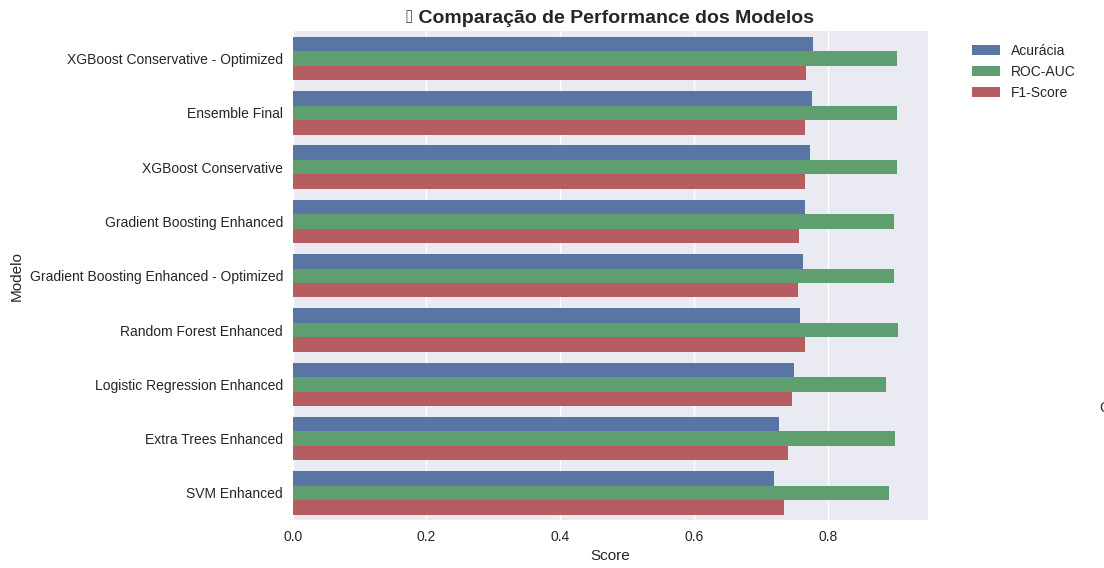
\includegraphics[width=1.07\textwidth]{images/comparacao_modelos.jpg}
\caption{Comparativo de Acurácia e F1-Score entre os modelos.}
\label{fig:comparacao_modelos}
\end{figure}

\begin{table}[h!]
\centering
\caption{Métricas de desempenho dos modelos de classificação.}
\label{tab:modelos}
\begin{tabular}{@{}lcccc@{}}
\toprule
\textbf{Modelo} & \textbf{Acurácia} & \textbf{ROC-AUC} & \textbf{F1-Score} & \textbf{CV Score (± std)} \\
\midrule
Random Forest      & 0.7593 & 0.9047 & 0.7654 & 0.7544 (±0.0063) \\
Gradient Boosting  & 0.7661 & 0.8995 & 0.7579 & 0.7624 (±0.0068) \\
\textbf{XGBoost}   & \textbf{0.7740} & \textbf{0.9043} & \textbf{0.7661} & \textbf{0.7660 (±0.0086)} \\
Extra Trees        & 0.7277 & 0.9005 & 0.7414 & 0.7485 (±0.0087) \\
Regressão Logística & 0.7503 & 0.8866 & 0.7474 & 0.7598 (±0.0133) \\
SVM                & 0.7198 & 0.8913 & 0.7342 & 0.7398 (±0.0125) \\
\bottomrule
\end{tabular}
\end{table}

Os modelos XGBoost e Gradient Boosting, que apresentaram os melhores resultados iniciais, foram submetidos a um processo de otimização de hiperparâmetros utilizando \texttt{GridSearchCV}. O modelo XGBoost otimizado alcançou uma acurácia de \textbf{0.7774}. Adicionalmente, um modelo de ensemble, combinando os três melhores classificadores via \texttt{VotingClassifier}, foi construído, atingindo uma acurácia de 0.7763.

\subsubsection{Análise do Modelo Final}
O modelo \textbf{XGBoost Otimizado} foi selecionado como o melhor preditor. O relatório de classificação detalhado, apresentado na Tabela~\ref{tab:class_report}, revela uma alta capacidade de predição para as classes "Graduate" (recall de 92\%) e "Dropout" (recall de 76\%). No entanto, o modelo apresentou dificuldade em identificar corretamente os alunos da classe "Enrolled", com um recall de apenas 41\%. A Figura~\ref{fig:matriz_confusao} ilustra a matriz de confusão do modelo, onde é possível observar visualmente esses acertos e erros.

\begin{table}[h!]
\centering
\caption{Relatório de Classificação do Modelo XGBoost Otimizado.}
\label{tab:class_report}
\begin{tabular}{lrrrr}
\toprule
\textbf{Classe} & \textbf{Precision} & \textbf{Recall} & \textbf{F1-Score} & \textbf{Support} \\
\midrule
Dropout    & 0.82 & 0.76 & 0.79 & 284 \\
Enrolled   & 0.55 & 0.41 & 0.47 & 159 \\
Graduate   & 0.81 & 0.92 & 0.86 & 442 \\
\midrule
\textbf{Accuracy} & & & \textbf{0.78} & \textbf{885} \\
\textbf{Macro Avg} & 0.73 & 0.70 & 0.71 & 885 \\
\textbf{Weighted Avg} & 0.77 & 0.78 & 0.77 & 885 \\
\bottomrule
\end{tabular}
\end{table}

\clearpage

% --- Inserir aqui a figura da Matriz de Confusão ---
% Exemplo de comentário:
\begin{figure}[h!]
\centering
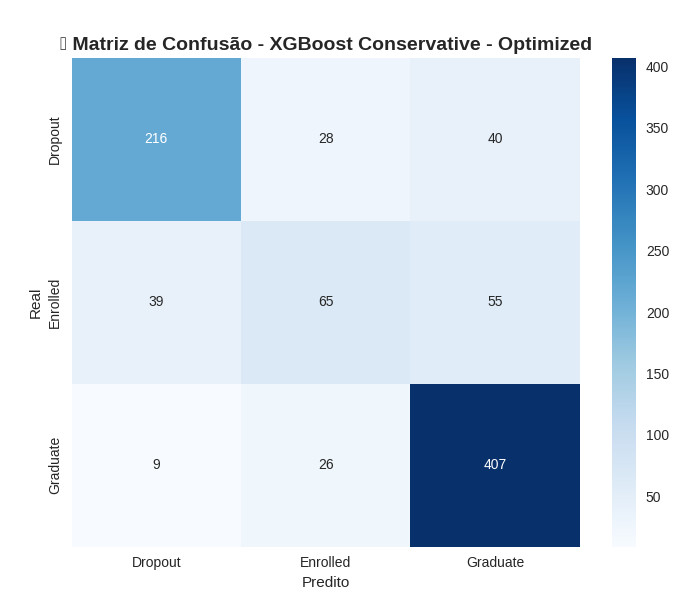
\includegraphics[width=0.6\textwidth]{images/matriz_confusao.jpg}
\caption{Matriz de Confusão do modelo XGBoost Otimizado.}
\label{fig:matriz_confusao}
\end{figure}

A análise de importância dos atributos revelou que a variável \texttt{approval\_rate} (taxa de aprovação) é, de longe, o fator mais preditivo, com um peso de 0.37, seguida por \texttt{Tuition fees up to date} (mensalidades em dia) e \texttt{Curricular units 2nd sem (approved)} (unidades aprovadas no 2º semestre), conforme destacado na Figura~\ref{fig:feature_importance}. Isso indica que o desempenho acadêmico contínuo e a situação financeira do aluno são determinantes para seu percurso na universidade.

% --- Inserir aqui a figura de Importância das Features ---
% Exemplo de comentário:
\begin{figure}[h!]
\centering
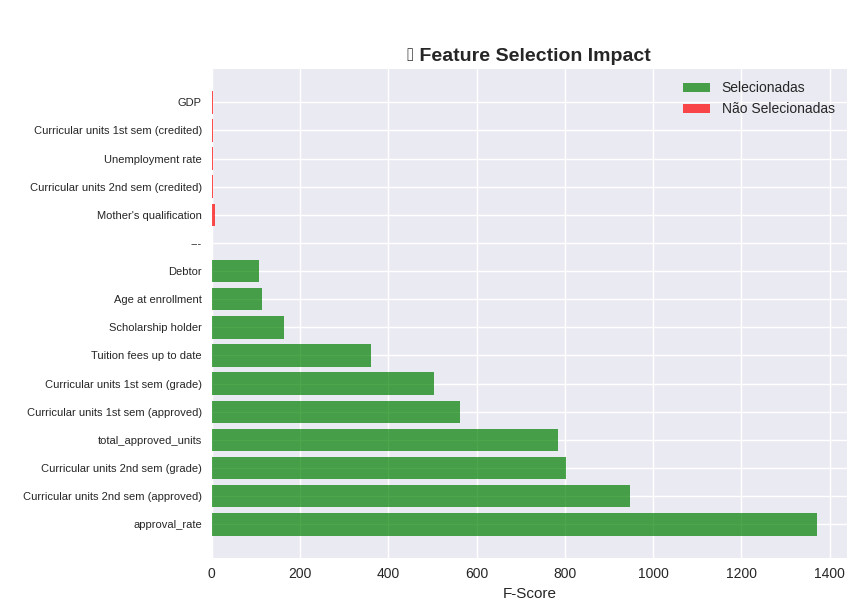
\includegraphics[width=1.0\textwidth]{images/feature_importance.jpg}
\caption{As 10 features mais importantes segundo o modelo XGBoost.}
\label{fig:feature_importance}
\end{figure}


\section{Conclusão}
Este trabalho demonstrou a viabilidade e a eficácia da aplicação de técnicas de Machine Learning para a análise e predição do desempenho acadêmico em instituições de ensino superior. O objetivo de desenvolver um modelo preditivo para identificar padrões e prever resultados futuros foi alcançado com sucesso.

O modelo final, baseado no algoritmo XGBoost, atingiu uma acurácia geral de aproximadamente 78\%, mostrando-se particularmente robusto na identificação de alunos com alta probabilidade de se graduarem (recall de 92\%) e daqueles em risco iminente de evasão (recall de 76\%). Estes resultados são promissores e fornecem uma base sólida para a implementação de ações preventivas.

A principal descoberta deste estudo reside na identificação dos fatores de maior impacto no percurso acadêmico. A "taxa de aprovação" (\texttt{approval\_rate}) emergiu como o preditor mais significativo, reforçando que o acompanhamento contínuo do rendimento do aluno é fundamental. Além disso, fatores como a regularidade no pagamento das mensalidades (\texttt{Tuition fees up to date}) e o número de unidades curriculares aprovadas no semestre anterior também se mostraram cruciais.

A principal limitação do modelo foi a baixa capacidade de prever com precisão a classe "Matriculado" (Enrolled). Isso sugere que este é um estado mais transitório e complexo, cujos fatores determinantes podem não ter sido totalmente capturados pelas variáveis disponíveis.

Com base nos resultados, as intervenções pedagógicas propostas na Etapa 4 podem ser direcionadas com maior precisão. Alunos que apresentem uma queda na taxa de aprovação podem ser rapidamente identificados e direcionados para programas de tutoria e reforço acadêmico. Da mesma forma, a importância do fator financeiro aponta para a necessidade de políticas de auxílio e suporte ao estudante.

Como trabalhos futuros, sugere-se a incorporação de novas fontes de dados, como informações comportamentais do ambiente virtual de aprendizagem (AVA) ou dados socioeconômicos mais detalhados, para aprimorar a predição da classe "Matriculado". Adicionalmente, a implementação deste modelo como uma ferramenta piloto no ambiente da universidade permitiria validar sua eficácia em um cenário real e refinar continuamente suas previsões, contribuindo para a redução das taxas de evasão e o aumento do sucesso acadêmico.
% --- Referências Bibliográficas ---
\renewcommand{\refname}{Referências}
\bibliographystyle{sbc}
\bibliography{sbc-template}
\end{document}
